\documentclass[8pt]{beamer}
\usepackage{tikz}
\usepackage[utf8]{vietnam}
\usepackage{amsmath}
\usepackage{graphicx}
\usepackage{mathrsfs}
\usepackage{amssymb,amsfonts,amsthm}
\usepackage{wrapfig}
\usepackage{hyperref}
\usetheme{Copenhagen}
\usecolortheme{spruce}
\setbeamertemplate{navigation symbols}{}
\setbeamertemplate{headline}{}
\setbeamertemplate{footline}{}
\title[Kết quả nghiên cứu tuần 2]
{Kết quả nghiên cứu tuần $2$}
\subtitle{Phòng thí nghiệm Thông tin Vô tuyến}
\author[Phòng thí nghiệm thông tin Vô tuyến]
{Tín Vũ}
\date[VLC 2021] % (optional)
{tinvu1309@gmail.com}
\begin{document}
\frame{\titlepage}
\begin{frame}{Mục lục}
\tableofcontents
\end{frame}
\begin{frame}{Tài liệu tham khảo}
\section{Tài liệu tham khảo}
Tài liệu tham khảo được sử dụng để nghiên cứu gồm: Antenna Theory (A.Balanis).
\end{frame}
\begin{frame}{Các tham số cơ bản của Antenna}
\section{Các tham số cơ bản của Antenna}
\begin{itemize}
	\item Beamwidth
\end{itemize}
\subsection{Beamwidth}
\begin{figure}[h]
			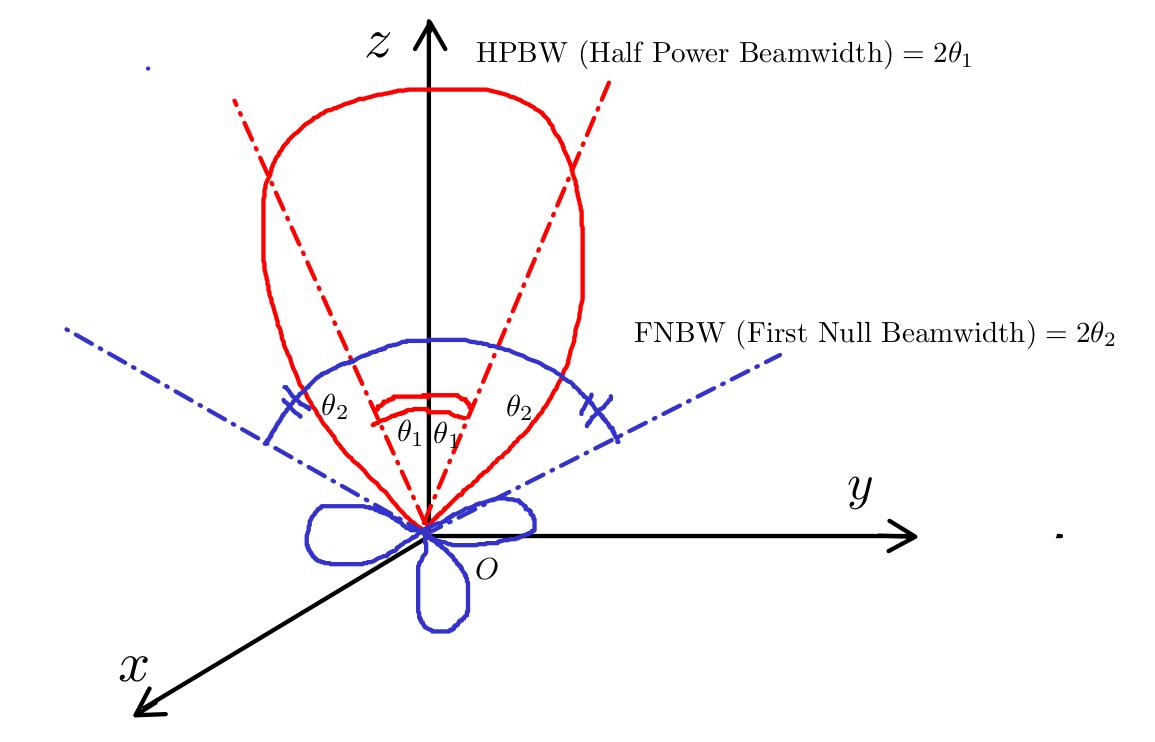
\includegraphics[width=0.9\textwidth]{beamwidth.jpg}
			\caption{Beamwidth model}			\label{fig:re1}
\end{figure}
\end{frame}
\begin{frame}{Các tham số cơ bản của Antenna}
 Theo IEEE, khái niệm "beamwidth" được định nghĩa là khoảng cách góc giữa hai điểm giống nhau đối xứng qua trục xác định.
\\ Trong quá trình thiết kế antenna, nếu giảm beamwidth thì side lobe tăng và ngược lại. 
\\ Ví dụ: Antenna có cường độ bức xạ chuẩn hóa được biểu diễn như sau: 
$$U(\theta)=\cos^{2}{\theta}\cos^{2}{3\theta} \quad \left(0\leq\theta\leq\frac{\pi}{2},0\leq\phi\leq 2\pi\right)$$
Hãy tìm HPBW và FNBW.
\\ Từ công thức $U=r^2 W$ đã được thảo luận ở slide trước, ta thấy $U,W,P$ là 3 đại lượng tỉ lệ thuận với nhau. Hiển nhiên ta có:
$$P(\theta_{h})=\frac{1}{2}P(\theta)\Leftrightarrow U(\theta_{h})=\frac{1}{2}U(\theta)=\frac{1}{2}$$
Giải phương trình lượng giác trên, ta thu được giá trị $\theta_{h}=0.25\;(rad)$, vậy ta có $\text{HPBW}=2\theta_{h}=0.5\;(rad)$. Hoàn toàn tương tự, ta cũng dễ dàng tìm được FNBW:
$$U(\theta_{f})=0$$
Ta thu được 2 nghiệm $\theta_{f1}=\frac{\pi}{6}\;(rad)$ và $\theta_{f2}=\frac{\pi}{2}\;(rad)$. Nghiệm đầu tiên $\theta_{f1}$ chính là nghiệm của FNBW:
$$\text{FNBW}=2\theta_{f1}=\frac{\pi}{3}\;(rad)\quad (\text{side lobe angular})$$
Nghiệm thứ hai $\theta_{f2}$ chính là nghiệm của SNBW (second null beamwidth):
$$\text{SNBW}=2\theta_{f2}=\pi\;(rad)\quad (\text{back lobe angular})$$
Các kết quả này hoàn toàn khớp với mô hình đã được trình bày ở trên.
\end{frame}
\begin{frame}{Các tham số cơ bản của Antenna}
\begin{itemize}
	\item Directivity
\end{itemize}
\subsection{Directivity}
Khái niệm "directivity" của antenna được định nghĩa là tỉ số giữa cường độ bức xạ tại một hướng với cường độ bức xạ tại mọi hướng (của một antennna đẳng hướng đã được phân tích ở slide trước).
$$D=\frac{U}{U_{0}}=\frac{U}{P_{rad}/(4\pi)}=\frac{4\pi U}{P_{rad}}$$
Trong hệ tọa độ cầu, chúng ta định nghĩa: $$D=D_{\phi}+D_{\theta}$$
với: 
\begin{equation*}
\begin{split}
	D_{\Phi}&=\frac{4\pi U_{\Phi}}{(P_{rad})_{\Phi}+(P_{rad})_{\theta}}\\
	D_{\theta}&=\frac{4\pi U_{\theta}}{(P_{rad})_{\Phi}+(P_{rad})_{\theta}}
\end{split}
\end{equation*}
\end{frame}
\begin{frame}{Các tham số cơ bản của Antenna}
\subsubsection{Ví dụ 1}
Ví dụ 1: xét một antenna có mật độ bức xạ:
$$W_{rad}=\hat a_{r}W_{r}=\hat a_{r}A_{0}\frac{\sin{\theta}}{r^2}\quad(W/m^2)$$
Với điều kiện bị giới hạn bởi mặt kín $S=\{(\phi,\theta)|0\leq\phi\leq2\pi,\;0\leq\theta\leq\pi\}$. Viết phương trình hàm $D(\phi,\theta)$ và tính $D_{max}(\phi,\theta)$.
Từ công thức: $$D=\frac{U}{U_{0}}=\frac{4\pi U}{P_{rad}}$$
Ta cần xác định $U$ và $P_{rad}$:
$$P_{rad}=\iint_{S}W_{rad}\hat a_{r}da=\iint_{S}W_{rad}\hat a_{r}r^2\sin{\theta}d\theta d\phi=\int_{0}^{2\pi}\int_{0}^{\pi}A_{0}\sin^2{\theta}d\theta d\phi=\pi^2A_{0}$$
$$U=r^2W_{rad}=A_{0}\sin{\theta}\Rightarrow D=\frac{4\sin{\theta}}{\pi}$$
Vậy ta có:
$$D(\phi,\theta)=\frac{4\sin{\theta}}{\pi}\Rightarrow D_{max}(\phi,\theta)=\frac{4}{\pi}$$

\end{frame}
\begin{frame}{Các tham số cơ bản của Antenna}
Ví dụ 2: thực hiện tương tự yêu cầu như ví dụ 1, nhưng với hàm mật độ bức xạ:

$$W_{rad}=\hat a_{r}W_{r}=\hat a_{r}A_{0}\frac{\sin^2{\theta}}{r^2}\quad(W/m^2)$$
Ta cần xác định $U$ và $P_{rad}$:
$$P_{rad}=\iint_{S}W_{rad}\hat a_{r}da=\iint_{S}W_{rad}\hat a_{r}r^2\sin{\theta}d\theta d\phi=\int_{0}^{2\pi}\int_{0}^{\pi}A_{0}\sin^3{\theta}d\theta d\phi=\frac{8\pi}{3}A_{0}$$
$$U=r^2W_{rad}=A_{0}\sin^2{\theta}\Rightarrow D=\frac{3}{2}\sin^2{\theta}$$
Vậy ta có:
$$D(\phi,\theta)=\frac{3}{2}\sin^2{\theta}\Rightarrow D_{max}(\phi,\theta)=\frac{3}{2}$$
\end{frame}
\end{document}
